\usetikzlibrary{calc}
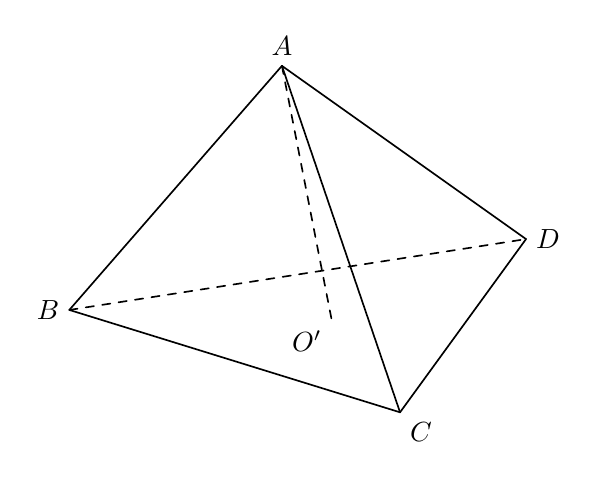
\begin{tikzpicture}[line width=0.6pt,line cap=round,line join=round]
\coordinate (A) at (2.700,5.600);
\coordinate (B) at (0.000,2.500);
\coordinate (C) at (4.200,1.200);
\coordinate (D) at (5.800,3.400);
\coordinate (Op) at (3.333,2.367);
\draw (A) -- (B);
\draw (A) -- (C);
\draw (A) -- (D);
\draw (B) -- (C);
\draw (C) -- (D);
\draw[dashed] (B) -- (D);
\draw[dashed] (A) -- (Op);
\node[above] at (A) {$A$};
\node[left] at (B) {$B$};
\node[below right] at (C) {$C$};
\node[right] at (D) {$D$};
\node[below left] at (Op) {$O'$};
\end{tikzpicture}
